\documentclass[10pt, a4paper, conference, compsocconf]{IEEEtran}

\usepackage{amssymb}

\usepackage[noend]{algpseudocode}

\makeatletter
\renewcommand{\ALG@beginalgorithmic}{\small}
\makeatother


\usepackage{algorithm}
\usepackage{colortbl}
\usepackage{color}

\usepackage{graphicx}
\graphicspath{{./figures/}}
\DeclareGraphicsExtensions{.eps}

\usepackage{tabularx}
\usepackage[footnotesize]{subfigure}

\newenvironment{definition}[1][Definition]{\begin{trivlist}
\item[\hskip \labelsep {\bfseries #1}]}{\end{trivlist}}

\usepackage{flushend}

\begin{document}

\title{A Multi-Objective Incremental Path Planning Algorithm for Mobile Agents}

\author{\IEEEauthorblockN{Tu\u{g}cem Oral}
\IEEEauthorblockA{Department of Computer Engineering\\
Middle East Technical University\\
06531, Ankara, Turkey\\
tugcem.oral@gmail.com}
\and
\IEEEauthorblockN{Faruk Polat}
\IEEEauthorblockA{Department of Computer Engineering\\
Middle East Technical University\\
06531, Ankara, Turkey\\
polat@ceng.metu.edu.tr}
}

\maketitle

\begin{abstract}
Path planning is a crucial issue in unknown environments where an autonomous mobile agent has to reach a particular destination from some initial location. There are several incremental algorithms such as D* \cite{DStar:1994}, D* Lite \cite{Koenig:2002} that are able to ensure reasonable paths in terms of path length in unknown environments. However, in many real-world problems we realize that path length is not only the sole objective. For example in computer games, a non-player character needs to not only find a minimum cost path to some target location but also minimize threat exposure. This means that path planning/finding activity of an agent in a multi-agent environment has to consider more than one objective to be achieved. In this paper, we propose a new incremental search algorithm called MOD* Lite extending Koenig's D* Lite algorithm and show that MOD* Lite is able to optimize path quality in more than one criteria that cannot be transformed to each other. Experimental results show that MOD* Lite is able to find optimal solutions and is fast enough to be used in real-world multi-agent applications such as robotics, computer games, or virtual simulations. 
\end{abstract}

\begin{IEEEkeywords}
Path planning; multi-objectivity; incremental search algorithm
\end{IEEEkeywords}

\section{Introduction}
The problem of finding a path for an autonomous agent from an initial location to a destination location is a popular problem in real-life applications including robotics, virtual simulations, computer games, etc. The path planning algorithms can be classified into three categories: off-line algorithms \cite{Dijkstra:1959} \cite{AStarHart:1968}, on-line algorithms \cite{RTAStarKorf:1990} and incremental algorithms \cite{DStar:1994}, \cite{Koenig:2002}, \cite{FocussedDStarStentz:1995}. Off-line path planning algorithms find the whole solution in advance before starting execution whereas on-line search algorithms require the planning and execution phases to be coupled, such that the agent repeatedly plans and executes the next move. In dynamic or partially known environments, off-line path planning algorithms suffer from execution time, whereas on-line algorithms yield low quality solutions in terms of path length. Incremental heuristic search algorithms try to merge advantages of both approaches to obtain better execution time without sacrificing optimality. They reuse the information gained from previous iterations and improve it instead of calculating from scratch like off-line search methods. 

Existing incremental algorithms for path planning problem attempt to minimize path length. However, in many real-life problem domains we see that there are several objectives to be optimized concerning the solution (path) quality. Consider the navigation of an unmanned vehicle from one coordinate to another on a 3D terrain in a warfare setting. The navigation task is defined to be finding a path which is shortest but also the most safest among all possibilities considering the existence of opponent forces in a partially known environment due to limited sensor capabilities. Note that shortest path may not be the safest one, but possibly the most dangerous one. And also the safest one may be the longest one which is unacceptable due to fuel consumption or time thresholds. 

There is a need to generalize the notion of quality of a path to meet specific requirements of complex application domains where several objectives (criteria) that cannot be transformed to each other exist. For example, in our unmanned vehicle example, it is not possible to transform the distance metric to safety metric, and vice versa. This requirement raises the problem of handling multiple criteria decision making. In this paper we introduce an incremental path finding algorithm, called Multi-Objective D* Lite (MOD* Lite) which extends D* Lite \cite{Koenig:2002}, an existing incremental algorithm. MOD* Lite can be used in the design of an autonomous mobile agent facing with the problem of navigation in a partially known environment that needs to optimize a predefined set of independent objectives (criteria). Agent can have limited sensor capability and hence partially observe the environment, and furthermore need to optimize multiple objectives at the same time. In order to show that MOD* Lite generates the optimal solutions we compared MOD* Lite against MOA* algorithm \cite{MOAStewart:1991}, an offline algorithm, on some test environments that are fully observable. We also tested the performance of MOD* Lite on several partially observable environments guaranteeing the optimal solutions but outperforming the MOA* version modified for unknown environments. 

The organization of the paper is as follows: Section II includes the background and related work on path planning. The problem definition and the characteristics of the environment are given in Section III. MOD* Lite and its details are given in Section IV. Section V presents test cases and experimental results. Concluding remarks and future research directions are provided in Section VI.

\section{Related Work}
In the literature, there are several algorithms focusing on path planning. In this section we would like to introduce existing research relevant to our study where the motivation is to handle existence of multiple objectives and partial observability in path planning. In that respect, we will highlight only multi-objectivity and incremental search here.

Multi-objective A* (MOA*) \cite{MOAStewart:1991} extends classical A* \cite{AStarHart:1968} to handle multiple objectives that inherently exist in many application domains. It uses the evaluation function $f(n)=g(n)+h(n)$ similar to A* but functions return vectors instead of scalar values. Size of the vector is the number of objectives to be optimized. If there is only one objective MOA* becomes standard A*. Like A*, it provides optimal solutions when heuristic function is admissible which means the heuristic estimation of every objective is not overestimated. MOA* keeps track of state expansions using {\it OPEN} and {\it CLOSED} sets. Non-dominated states are maintained in a subset of {\it OPEN} named {\it ND}. At each iteration of the algorithm, the best alternative is selected from {\it ND} and expanded until it becomes empty. Finally, solution paths are generated by following back-pointers from goal to start. 

Bayili and Polat introduced a multi-objective path planning algorithm, Limited Damage A*  \cite{LDAStarBayili:2008} considering damage as a feasibility criterion in addition to distance. When an agent navigates in a threat zone, it is exposed to an additive damage. An upper bound is predefined for maximum damage that can be exposed and the algorithm discontinue the search on paths with damage score exceeding this threshold. The algorithm was shown to find suboptimal solutions with a reasonable time performance compared to MOA*. 

Tarapata presented multi-objective approaches to shortest path problems in his study \cite{Tarapata:2007}. He gave a classification of multi-objective shortest path (MOSP) problems and discussed different models of them. Also he presented methods of solving the formulated optimization problems. Analysis of the complexity of the presented methods and ways of adapting of classical algorithms for solving MOSP problems were described in detail. The comparison of the effectiveness of solving selected MOSP problems were defined as mathematical programming problems and multi-weighted graph problems. Experimental results of using the presented methods for multi-criteria path selection in a terrain-based grid network were given. Guo et al. concentrated on the problem of multi-objective path planning (MOPP) for the ball and plate system in \cite{Guo:2009}. The goal of MOPP was to obtain the safe -without colliding hazardous obstacles- and shortest path for the ball to follow. The environment was represented by distance and hazard map which represents possible collisions between the ball and the obstacles. They used an entropy-based method to calculate weights of objectives for each grid node. In simulation results, the path obtained by multi-objective method was much safer compared with single-objective A* algorithm. 

Evolutionary methods were also proposed for multi-objective path planning. A recent study by Pangilinan et al. \cite{Pangilinan} has introduced an evolutionary algorithm for multi-objective shortest path problem and their results show that the algorithm is a good alternative in finding a subset of efficient solutions for multi-objective shortest path problems when performance issues like complexity, diversity and non-dominal optimal solutions become obstructions. Castillo et al. also worked on evolutionary algorithms for MOPP in \cite{Castillo:2007}. They defined a genetic offline point-to-point agent path planner works on 2-D static grid environment. Bukhari et al. came up with an optimization technique for dynamic on-line path planning in \cite{Bukhari:2010} using particle swarm optimization. The proposed algorithm generated and optimized paths in complex and large environments with several constraints. Complete discussion of multi-objective evolutionary algorithms (MOEA) can be found in \cite{MOOUEA}.

Algorithms on incremental search aim to generate an initial sub-optimal path, and try to improve it during the consequent iterations to make it closer to the optimal. Stentz et al. proposed the Dynamic A*, D* \cite{DStar:1994} which guarantees to be optimal and is functionally equivalent to re-planning from scratch. Later, D* Lite was proposed by Koenig et. al \cite{Koenig:2002} which utilized the same navigation strategy with D* but algorithmically different. It was based on Lifelong Planning A* (LPA*) \cite{LPAStarKoenig:2004}. D* Lite basically works as A* in the first iteration, then only updates for changed weights in environment. They prove that D* Lite was at least as efficient as D*. 

\section{Problem Definition \& Environment}
\subsection{Definition of the Problem}
Consider that an unmanned aerial vehicle (UAV) is landing off from an initial location. Its goal is trying to shoot an enemy unit on a predefined target location in an unknown dynamic environment. However, this enemy unit is protected by air defense units scattered on the terrain having different capabilities (hit ratios) and coverage areas. Each defense unit scans the space within its coverage areas to detect any threat. Due to its limited sensor capability, a UAV can only partially observe the environment. The air defense zones produce computable risk values for UAVs when they enter UAV's perceived sensor range. On the other hand; UAV has limited fuel and time, so it must locate and shoot the target but the risk of being hit by an air defense unit must be minimized. This means that the UAV should both find a shortest and safest path \textit{as fast as possible}. 

In this real-world problem, the UAV has to execute a planner and quickly find available paths. Also it must re-plan its path quickly when a part of the environment become known as it navigates. Evolutionary search algorithms focus on this issue and come up with several solutions \cite{Peng_Xu_Zhang:2011}, \cite{Foo_Knutzon:2009}. It is obvious that existing algorithms are insufficient for reflecting the dynamics of the environment as they are not incremental. One alternative could be to adapt off-line MOA* to unknown environments but it is grossly inefficient as it has to be restarted from scratch every time some part of the environment becomes known. 

Our algorithm MOD* Lite enables a user to define a set of objectives, $O_1, O_2, \cdots, O_n$ to be used in the evaluation of the quality of the candidate paths explored by an incremental algorithm. In that respect MOD* Lite is a domain-independent path search algorithm that can be used in any search problem where the environment is partially or fully observable. Note that for each objective $O_i$, the user needs to define whether $O_i$ is to be minimized or maximized. For the sake of simplicity, we restrict ourselves to the UAV domain we have just introduced above and presume the existing of two objectives to be minimized, namely the distance and the degree of danger.

\subsection{Environmental Properties}
\label{envPropertiesSSection}
We illustrate MOD* Lite applied to the UAV path finding task in a 2-D grid based environment. It is easier to present the algorithm and also demonstrate its effectiveness on a such simple environment. 

The environment is considered to be partially observable because of limited sensor capability of the agent. The agent can perceive the environment around him/her within a square region centered at the agent location. The size of the square is $(2v + 1)$ x $(2v + 1)$, where $v$ is the vision range. As the agent navigates, the known part of the environment gradually increases and we presume that agent has enough memory space to maintain the environment. It is assumed that the target is stationary and its location is known by the UAV agent at the initial step. Furthermore, the environment has randomly placed obstacles that cannot be crossed over by the agent. The agent occupies only one grid cell. There are also threat zones in the environment. Threat zones produce predefined risk values which could effect the agent to fail reaching to the target cell. Threat zones are constructed up to three sub-zones. The innermost one is more hazardous than outer ones. So, if agent has to enter a threat zone, it prefers to pass through outer levels. With threat zones, agent must both think about the shortest and the safest path. The environment has randomly placed different sized threat zones.

\section{MOD* Lite}
\subsection{Overview}
Multi-objective problems focus on considering more than one objective at the same time. Consequently, \textit{all} scalar values and atomic operations (like addition, checking for equality, etc.) are to be adapted into vectors of scalars. This causes cost functions to have $n$ dimensions if there are $n$ \textit{non-interacting} objectives to be optimized. For two scalars a and b, there are three outcomes: $a<b$, $a>b$ or $a=b$. However for two vectors $u$ and $v$, besides $u<v$, $u>v$ and $u=v$ we have a fourth alternative meaning that $u$ and $v$ cannot be compared. $u$ and $v$ are said to be equal if the corresponding objective values are equal. We say that $u$ \textit{dominates} $v$ if $u$ is better in at least one objective compared to $v$ or in other words, there is no objective of $v$ where it is better than any objective of $u$. Moreover, $u$ and $v$ are said to be {\it non-dominated} if for at least one objective $u$ is better but for at least some other objective $v$ is better. For instance, assume that we have two objectives to be minimized and let $\upsilon_{1}=[3,4], \upsilon_{2}=[4,6], \upsilon_{3}=[6,2] $. Here $\upsilon_{1}$ dominates $\upsilon_{2}$ but $\upsilon_{1}$ and $\upsilon_{3}$ are non-dominated.

\subsection{The Components and Variables}
MOD* Lite is the multi-objective extension of D* Lite. It can be applied to any unknown dynamic multi-objective search problem where costs can change by time. Considering formal definition; $S$ denotes the set of states in search problem. $s_{start} \in S$ and $s_{goal} \in S$ are the initial and final (target) states, respectively. $pred(s) \subseteq S$ and $succ(s) \subseteq S$ can be used to find predecessors and successors of given state, $s$. The heuristic function $h(s, s')$ which estimates costs between $s$ and $s'$, cost function $c(s, s')$ which represents the actual cost traversing from $s$ to $s'$, actual cost function $g(s)$ and the $rhs(s)$, one-step-lookahead values of $g(s)$ functions are inherited from D* Lite. However, as we have to consider more than one objective, these functions are to return vectors of scalars instead of scalars. Thus, $rhs(s)$ satisfies the condition

\begin{footnotesize}
\[ rhs(s) = \left\{ \begin{array}{cc}
ObjectiveVector.MIN & \mbox{if $s=s_{start}$};\\
nonDom_{s' \in pred(s)}(sum(g(s'), c(s', s))) & \mbox{otherwise}.\end{array} \right. \] 
\end{footnotesize}

where ObjectiveVector.MIN stands for a vector with $n$ minimum values for $n$ dimensional problem. These values could be $0$ or $\infty$ for minimization or maximization of objective, respectively. $sum()$ function implements vector summation and $nonDom()$ function returns the set of best non-dominated vectors corresponding to predecessors of any state $s$. Note that $nonDom()$ constructs a list of objective vectors, $rhs(s)$ and $g(s)$ function values are represented as a \textit{lists of objective vectors} where each objective vector in this list is non-dominated with others. An objective vector is a structure that holds values for each objective defined by problem (minimization or maximization). In case of having more than one objective, it is possible that there are more than one paths to a particular state that do not dominate each other. That's why we may have several vectors for any state. In case we need to compare whether one state is better than another, we need to compare two sets of vectors, as formulated below.

\begin{definition}
$u$ \textit{completely dominates} $v$ iff $\forall x\in u$ $\forall y\in v\;$ $x$ dominates $y$.
\end{definition}

Assume that $\upsilon_{1}=\{[2,5],[3,4]\}, \upsilon_{2}=\{[6,1],[5,2]\}, \upsilon_{3}=\{[3,5]\}$ are lists of objective vectors for three states. $\upsilon_{1}$ and $\upsilon_{2}$ are non-dominated whereas $\upsilon_{1}$ completely dominates $\upsilon_{3}$. 

We could frankly say that the terms "greater than", "smaller than" and "equals" for scalar value comparison are replaced by "completely dominates", "completely dominated by" and "multi-objectively equals" for vectors of scalars. Non-domination is introduced and handled as the fourth case.

D* Lite introduces local consistency and inconsistency concepts with respect to comparing $g(s)$ and $rhs(s)$. A state is called {\it locally consistent} when $g(s)$ and $rhs(s)$ are equal or {\it locally inconsistent} otherwise. A locally inconsistent state is referred as locally underconsistent if $g(s)<rhs(s)$ or locally overconsistent if $g(s)>rhs(s)$. In the case of non-domination of these functions, we introduce the concept of {\it local non-consistency}:

\begin{definition}
A state is referred as \textit{locally non-consistent} if its $g(s)$ and $rhs(s)$ values are non-dominated to each other. This inconsistency condition causes the state resides on more than one solution because it can be understood that two or more predecessors of $s$ are non-dominated to each other.
\end{definition}

Other multi-objective operations we use are introduced in following subsections. The overall flow of MOD* Lite is given in Algorithm \ref{algMain}.

%% The main algorithm.
\begin{algorithm}
	\caption{Main loop of MOD* Lite}
	\label{algMain}
	%\begin{spacing}{0.5}
	{\fontsize{9}{9}\selectfont
    \begin{algorithmic}[1] % line numbering every line
      \Function{calculateKey}{s}
      	\State $k_{2}$(s)= nonDom(g(s), rhs(s))
      	\State $k_{1}$(s) = sum(h($s_{start}$, s), $k_{m}$, $k_{2}$(s))
      	\State \Return $[k_{1}(s), k_{2}(s)]$
      \EndFunction
   	  \Statex
      \Function{initialize()}{}
      	\State $U = \varnothing $
      	\State $k_{m}$ = ObjectiveVector.MIN
      	\ForAll{$s \in S$}
     		\State rhs(s)=g(s)=ObjectiveVector.MAX
     	\EndFor
      	\State rhs($s_{goal}$) = ObjectiveVector.MIN
      	\State U.insert($s_{goal}$, calculateKey($s_{goal}$))
	  \EndFunction
	  \Statex
	  \Function{plan()}{}
      	\State initialize()
      	\State computeMOPaths()
      	\While{$true$}
    	      	\State solutionPaths = generateMOPaths()
    	      	\If{solutionPaths = null} there is no known path \EndIf
    	      	\State Wait for any weight cost to change;
    	      	\If{Any weight cost changes}
    	      		\State $k_{m}$ = sum($k_{m}$, h($s_{goal}$, $s_{start}$))
    	      		\ForAll {Changed weight costs of edges(u,v)}
    	      			\State Update cost c(u,v)
    	      			\State updateVertex(u)
    	      		\EndFor
		      	\State computeMOPaths()
    	      	\EndIf
		\EndWhile
  	  \EndFunction
    \end{algorithmic}}
    %\end{spacing}
\end{algorithm}

\begin{figure}
\centering
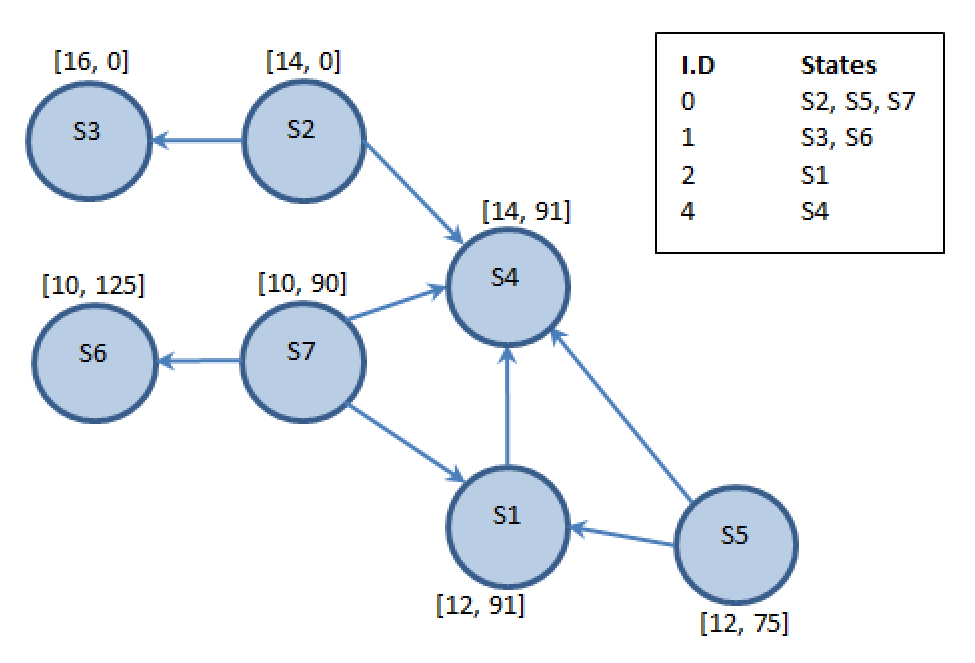
\includegraphics[width=2.3in]{graph1v2}
\caption{Directed Acyclic State Expansion Graph}
\label{fig:graph1}
\end{figure}

Basically, D* Lite tries to make all states locally consistent. Locally inconsistent states are maintained in  a priority queue (U) with their key values and expanded considering priority values. However, locally non-consistent states cannot be maintained in such a queue due to the non-domination of their key values, which are also set of objective vectors. If two keys cannot be dominated by each other, they should be criticized in the same manner. Thus, we come up with a more convenient structure, a directed acyclic state expansion graph instead priority queue which uses topological ordering of states with respect to the key domination. In this model, the graph (U) contains set of nodes each represented with a state and its key value. When a state is to be added into U with $insert(state, key)$ operation, key value is compared with all existing nodes' key values. If the new state dominates some state, an edge is introduced from the new state to this state. No edge is introduced in case of equality and non-domination. As a result, incoming and outgoing degrees of a node $s$ correspond to the number of nodes \textit{dominated by} $s$  and the number of nodes that $s$ \textit{dominates}, respectively. The node(s) with incoming degree 0 are the non-dominated nodes where none of other nodes could dominate. $topKey()$ and $topKeys()$ return the key value(s) of nodes with minimum incoming degree. $pop()$ returns and removes the state (all its incident -incoming and outgoing- edges are also removed from the graph) with minimum incoming degree. If more than one nodes exist with minimum degree, one of them is selected randomly. $remove(state)$ operation removes a given state and its incident edges from graph. An example of a state expansion graph with states and their corresponding key values is given in Figure \ref{fig:graph1}. Incoming degrees of nodes are given as a list in the figure.

Addition of a new state to the state expansion graph is illustrated in Figure \ref{fig:graph2}.  $S8$ is  "the new" state to be added, the dashed directed edges are established between $S8-S1$, $S8-S4$ and $S8-S5$ because $S8$'s key can only dominate keys of nodes $S1, S4$ and $S5$. None of the existing states' keys can dominate $S8$, so incoming degree of $S8$ becomes 0. This addition also effects the incoming degrees list where the changed positions are highlighted in the figure. Addition of $S8$ increments the incoming degrees of $S1$, $S4$ and $S5$ by 1 so their positions are shifted down.

\begin{figure}
\centering
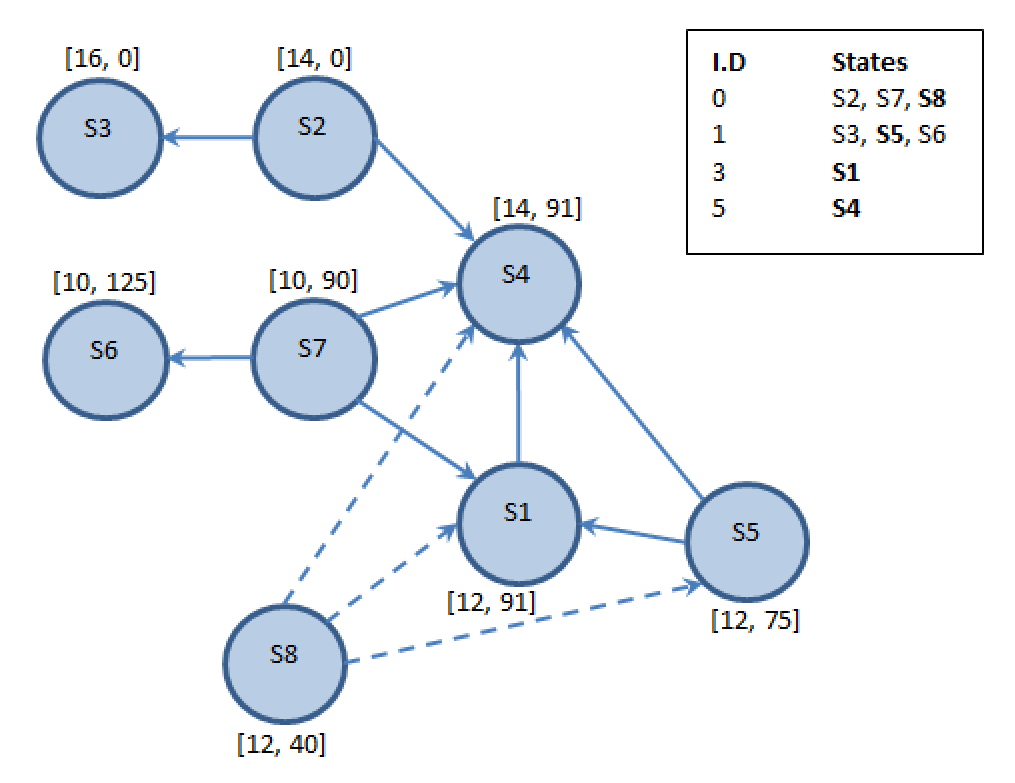
\includegraphics[width=2.3in]{graph2v2}
\caption{State Expansion Graph after Adding State $S8$}
\label{fig:graph2}
\end{figure}

\subsection{Key Formulation}
In the previous subsection, we state that the directed acyclic graph structure is used to determine expansion of nodes in state space with their \textit{keys}. The basic idea behind the calculation of keys is similar with D* Lite, with slight modifications. As we consider the algorithm in a multi-objective setting, key value is stated as a vector with two components: $k(s) = [k_{1}(s);k_{2}(s)]$ where these components are set of objective vectors. $k_{2}(s)$ is calculated by finding the \textit{non-dominated list} of $g(s)$ and $rhs(s)$, $k_{2}(s)= nonDom(g(s), rhs(s))$. The other component, $k_{1}(s)$  is calculated as vector summation of $h(s_{start}, s), k_{m}$ and $k_{2}(s)$. Calculation of $k(s)$ can be seen in lines \{2 and 3\} in Algorithm \ref{algMain}. $k_{m}$ is used for heap reordering as defined in  D* Lite.

\begin{algorithm}
	\caption{Update Vertex \& Compute Multi-Objective Paths}
	\label{algUpdate}
    \begin{algorithmic}[1]
   	  \Function{updateVertex}{u}
   	  	\If{$u \neq s_{goal}$}
   	  		\State $rhs(u) = nonDom_{s' \in succ(u)}(sum(c(u,s'), g(s')))$
   	  	\EndIf
   	  	\If{$u \in U$} U.remove(u) \EndIf
   	  	\If{!equals(g(u), rhs(u))}
   	  		\State U.insert(u, calculateKey(u))
   	  	\EndIf
   	  \EndFunction
    	  \Statex
      \Function{computeMOPaths()}{}
		\While{dominatesAll(calculateKey($s_{start}$), U.topKeys())}
		% OR !equals(rhs(s_{start}, g(s_{start}))$}
			\State $k_{old}$ = U.topKey()
	      	\State u = U.pop()
	      	\State $k_{new}$ = calculateKey(u)
	      	\If{$k_{old}$.completelyDominates($k_{new}$) }
	      		\State U.insert(u, $k_{new}$)
	      	\ElsIf{rhs(u).completelyDominates(g(u))}
	      		\State g(u) = rhs(u)
	      		\ForAll{$s \in pred(u)$} $updateVertex(s)$ \EndFor
	      	\ElsIf{g(u).completelyDominates(rhs(u))}
	      		\State g(u) = ObjectiveVector.MAX
	      		\ForAll{$s \in pred(u) \cup \{u\}$} $updateVertex(s)$ \EndFor
	      	\Else
	      		\State g(u) = nonDom(g(u), rhs(u))
	      		\ForAll{$s \in pred(u)$} $updateVertex(s)$ \EndFor
	      	\EndIf
		\EndWhile
	  \EndFunction
	\end{algorithmic}
\end{algorithm}

\subsection{Details of MOD* Lite}
MOD* Lite is based on  D* Lite algorithm as introduced in the previous section. There are fundamental differences due to the structures used and the way the solution paths are maintained. The pseudocode of MOD* Lite is given in Algorithms \ref{algMain}, \ref{algUpdate} and \ref{algPathGen}.

Searching order of MOD* Lite is from goal to start state, like D* Lite. The main function of MOD* Lite first calls $initialize()$ to setup the execution in Algorithm \ref{algMain}. This function calculates the key value for goal state, adds it into U and sets the rhs value to a \textit{MIN} objective vector, which has n values for n-objectives. These values can be $0$ for minimized-objective and $\infty$ for maximized-objective. Then, proper $g(s)$ values are calculated considering all objectives with $computeMOPaths()$. Finally, paths are generated with these $g(s)$ values. If a weight cost is changed in the environment, corresponding states are re-expanded and only related weights are updated. Notice that this cost change might happen for only one objective or several objectives at the same time.

The $computeMOPaths()$ pseudocode is given in Algorithm \ref{algUpdate} line \{7\}. The termination criteria of this function is where the key of $s_{start}$ dominates all the top keys returned from U. Until it terminates, the top state is sequentially selected from top states of U and expanded. While expanding a state, the domination between g and rhs values of corresponding state is observed. If $rhs(s)$ values completely dominate $g(s)$ values, local underconsistency case occurs. We apply the same strategy with D* Lite, update g value with rhs and update weight for all predecessors of s with $updateVertex()$. If $g(s)$ values completely dominate $rhs(s)$ values, the case is locally overconsistency. Simply g value for this state is set as \textit{MAX} objective vector, which is $\infty$ for minimized-objective and $0$ for maximized one and current state weight is updated with its predecessors' weight. The third case occurs when g and rhs values can not completely dominate each other, locally non-consistency. In this case, g value is updated with non-dominated values of g and rhs values and again predecessors of current state is updated. Keeping non-dominated values of g and rhs enables to keep track of each non-dominated successors' information.

To update a weight of a state, MOD* Lite uses $updateVertex(u)$ shown in Algorithm \ref{algUpdate} line \{1-6\}. It simply adds corresponding state to or removes from U according to given criteria. While updating $rhs(u)$ except goal state, non-dominated objective values of multi-objectively summed $c(u,s')$ and $g(s')$ are established and used.

After state expansion operation finalized and corresponding $g(s)$ values are set, multi-objective paths are generated via these $g(s)$ values by given pseudocode in Algorithm \ref{algPathGen}. Path generation is achieved in two phases: setting parent(s) for each non-dominated successor of expanding state and constructing paths by following these parents. The first phase is performed from the start to the goal state whereas the second is from the goal to the start state. 

A queue is used to keep track of expanding states. This queue initially has $s_{start}$ only, as shown in line \{2\}. Thus, starting from $s_{start}$, the while loop iterates until this queue becomes empty. Finding a goal state is not considered on termination criteria because other non-dominant paths might be available. As expanding a state, we refer to set \textit{it} as a parent to its successors indicated between lines \{7-39\}.

Before expansion of a state $s$, non-dominated successors are found first with respect to multi-objective summation of $c(s,s')$ and $g(s')$ as shown in line \{5\}. If a successor $s'$ is found in non-dominated successors list, it has a potential to have $s$ as a parent. For each non-dominated successor $s'$, first parents list of $s$ is checked. If $s$ does not have any parent, which only occurs iff $s=s_{start}$, for sure $s'$ does not have any parent as well. In this case, $s$ is added  as a parent of $s'$ with corresponding cost $c(s,s')$. Parents of a state are kept in a map where keys of this map are parents and values are cumulative costs which is consumed to reach that state from start through corresponding parent. These costs are used to determine elimination of existing parents when a new one is considered to add. We will elaborate this idea later.

% Indentations are used make visualization better.
\begin{algorithm}
	\caption{Path Generator Algorithm}
	\label{algPathGen}
    \begin{algorithmic}[1]
    		\Function{generateMOPaths()}{}
			\State expandingStates.add($s_{start}$)
    			\While{!expandingStates.isEmpty()}
    				\State s = expandingStates.poll()
				\State nonDomSuccs = $nonDom_{s' \in succ(s)}$(sum(c(s, s'), g(s'))
    				\ForAll{$s'\in nonDomSuccs$}
    					\If{s.parents() = null}
    						\State s'.parents().put(s, c(s, s'))
    					\Else
    						\State cumulativeC = sum(c(s, s'), s.parents().values())
    						\If{s'.parents() = null}
    							\State s'.parents().put(s, cumulativeC)
    						\Else
							\ForAll {$s'' \in s'.parents()$}
								\If{equals(s'.parents(s''), cumulativeC) OR completelyDominates( s'.parents(s''), cumulativeC)}
									\State \textbf{break}
								\ElsIf{completelyDominates(cumulativeC, 
								\\ \ \ \ \ \ \ \ \ \ \ \ \ \ \ \ \ \ \ \ \ \ \ \ \ \ \ s'.parents(s''))}
									\State s'.parents().remove(s'')
									\State s'.parents().put(s, cumulativeC)
								\Else
									\ForAll{$cC \in cumulativeC$}
										\ForAll{$eC \in s'.parents(s'')$}
											\If{eC.equals(cC) OR
											\\ \ \ \ \ \ \ \ \ \ \ \ \ \ \ \ \ \ \ \ \ \ \ \ \ \ \ \ \ \ \ \ \ \ \ \ \ \ \ \ eC.dominates(cC)}
												\State cumulativeC.remove(cC) 
												\State \textbf{break}
											\ElsIf{cC.dominates(eC)}
												\State s'.parents(s'').remove(eC) 
												\State \textbf{break}
											\EndIf
										\EndFor
										\If{s'.parents(s'') = null}
											\State s'.parents().remove(s'')
										\EndIf
									\EndFor
									\If{!cumulativeC = null}
											\State s'.parents().put(s, cumulativeC)
									\EndIf
								\EndIf
							\EndFor    						
    						\EndIf
    					\EndIf
    					\If {s'.parents.contains(s) AND \\ \ \ \ \ \ \ \ \ \ \ \ \ \ !expandingStates.contains(s')}
    						\State expandingStates.add(s')
    					\EndIf
    				\EndFor
    			\EndWhile
    			\State solutionPaths = construct paths recursively traversing parents
    			\State \Return solutionPaths
    		\EndFunction
	\end{algorithmic}
\end{algorithm}

If $s$ has predefined parents (starting from \{9\}), a cumulative total cost is calculated for $s'$ in line \{10\}. This cost is multi-objective summation of $c(s, s')$ and aggregated cost values of parents of $s$. Notice that the algorithm proves that parents' costs of a state are always non-dominated to each other, so the aggregated cost values contain \textit{all} parents' \textit{all} costs. These cost values express all non-dominated solution costs to reach that state. If $s'$ does not have any parent up to now (\{11\}), $s$ is added as a parent of $s'$ with cumulative cost. Else, each existing parent of $s'$, say $s''$ should be compared with the cumulative cost. These operations are shown in lines between \{13-34\}. Here, if $s''$ has same cost with or better cost (determined by completely domination term) than cumulative cost, needless to say that $s$ is not required to add as a parent to $s'$. Otherwise, if cumulative cost completely dominates $s''$, it can be inferred that one can reach to $s'$ from $s$ in a better way than $s''$. Thus, $s''$ is removed from parents of $s'$ and $s$ is added with the cumulative cost. The fourth possibility occurs when costs of $s''$ and cumulative costs can not completely dominate each other. In this situation, each cost in cumulative costs is compared with each cost of $s''$ costs. Equality or domination probabilities causes to remove corresponding cost from its list. At the end of the comparison, $s''$ is removed from parents of $s'$ if all of its costs are dominated (lines \{31-32\}) and $s$ is added as a parent if cumulative costs still have non-dominated cost (lines \{33-34\}).

After organizing parents of $s'$, it is decided to expand it in next iterations. If $s$ is successfully added as a parent and expanding states queue already does not have it, $s'$ is added to the tail of the queue. This can be seen in lines \{35-37\}.

When all non-dominated parents are properly set from start to goal state, these parents can be followed recursively starting from goal towards start state and multi-objective paths are constructed. Finally, all found paths have non-dominated path costs regarding to each other.

\section{Experimental Results}
\label{expResultsSection}

MOD* Lite is a domain independent algorithm and can be applied to any virtual environment with given $n$ objectives, whether \textit{maximized} or \textit{minimized}. The vital assumption about objectives is their independency to each other. If two objectives could effect each other in a positive or negative manner, this might reduce or expand objectives vector size, which is out of this study' s scope. Thus, we assume that each defined objective is considered in different perspective and can not be transferred to each other.

MOD* Lite algorithm is tested on various environments with different scenarios and compared to MOA* that guarantees optimal solutions in fully known environments. However, as it is not possible to exemplify all possible cases, specific and several extreme conditions are selected for experiments. First, our aim is to show that MOD* Lite is complete and optimal in fully observable environments. The performance comparison is done in two dimensions, execution times and paths they generate (path quality), respectively. Both algorithms are implemented in Java and run under Linux environment which has Intel Core2 Quad CPU with 2.33GHz and 4 GB RAM.

We generate partially and fully observable 2-D grid environments as detailed in subsection \ref{envPropertiesSSection} in our tests. The agent tries to find available non-dominated best paths using two objectives, path length and risk taken from threat zones. Thus, the agent endeavors to minimize both objectives and tries to find \textit{shortest} and \textit{safest} paths in all environments used in tests. In the first set of tests, randomly generated maps with different sizes  25 x 25, 50 x 50, 75 x 75, 100 x 100, 125 x 125 and 150 x 150, are used. In this test group, maps are taken as fully observable. Each of these maps have nearly 30\%-32\% threat zone and 14\%-16\% obstacle ratio. Agent's initial and target locations are also taken randomly. For this case, execution times and generated paths' costs of different sized maps are given in Figure \ref{fig:rand_fully} and Table \ref{table:randPaths}. As seen from results, MOD* Lite finds optimal and sub-optimal results while a gradually increases on time manner. Notice that taken risk values depend on environmental properties and should not be compared between different size of maps.

\begin{figure}
\centering
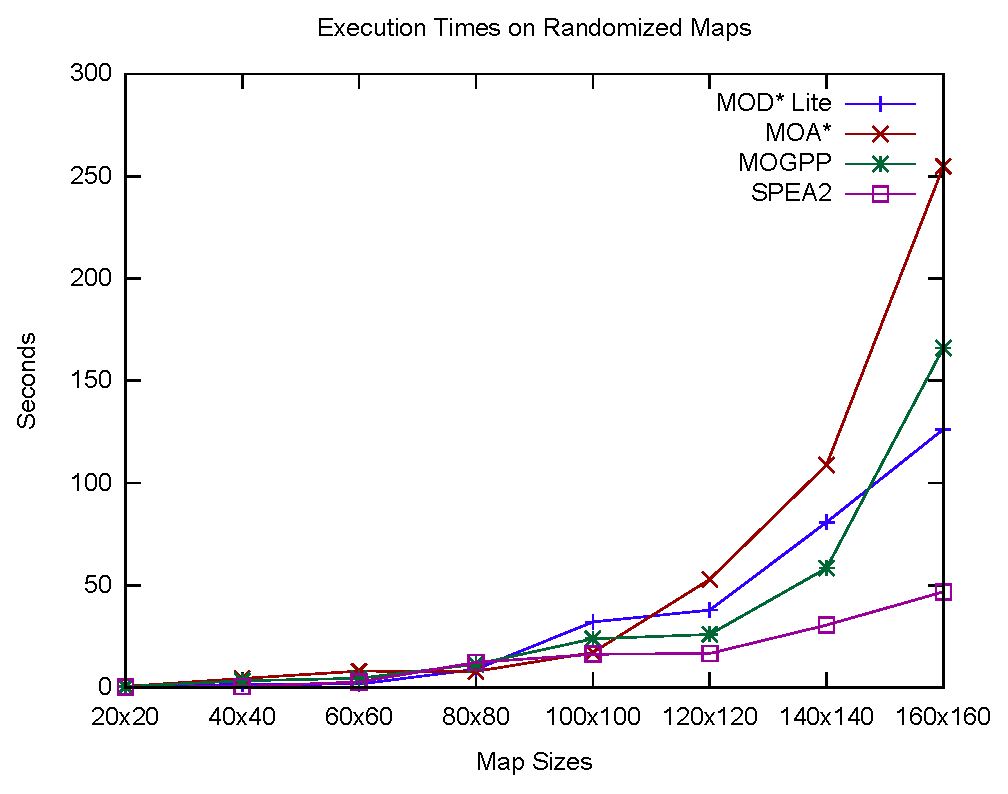
\includegraphics[width=2.1in, angle=270]{randomized}
\caption{Execution Times of Randomly Generated Fully Observable Maps}
\label{fig:rand_fully}
\end{figure}

\begin{table}[ht]
	\caption{Found Non-dominated Path Costs For Randomized Maps} % title of Table
	\centering
    \begin{tabular}{l l l}
        \hline
        Map Size  &  MOD* Lite  &  MOA* \\ [0.5ex] \hline
        25 x 25   &  (49, 571)  &  (49, 571) 
		   \cr    &  (51, 10)   &  (51, 10) \\ 
        50 x 50   & (99, 982)   & (99, 982)
		   \cr	  &	(101, 0)   &  (101, 0) \\ 
        75 x 75   & (149, 1549) & (149, 115) 
		   \cr	  &  (151, 221) & (153, 0)
		   \cr	  &  (153, 0)	&	\cr
        100 x 100 & (199, 10) & (199, 10)
		   \cr    & (201, 4) & (201, 4)
		   \cr    & (203, 0) & (203, 0) \\ 
        125 x 125 & (90, 1036) & (90, 1036) 
		   \cr	  & (92, 293) & (92, 293)
		   \cr	  & (94, 165) & (94, 165)
		   \cr	  & (96, 101) & (96, 101) \\
        150 x 150 & (126, 128) & (126, 128) \\ [1ex]
        \hline
    \end{tabular}
	\label{table:randPaths}
\end{table}


\begin{figure}
\centering
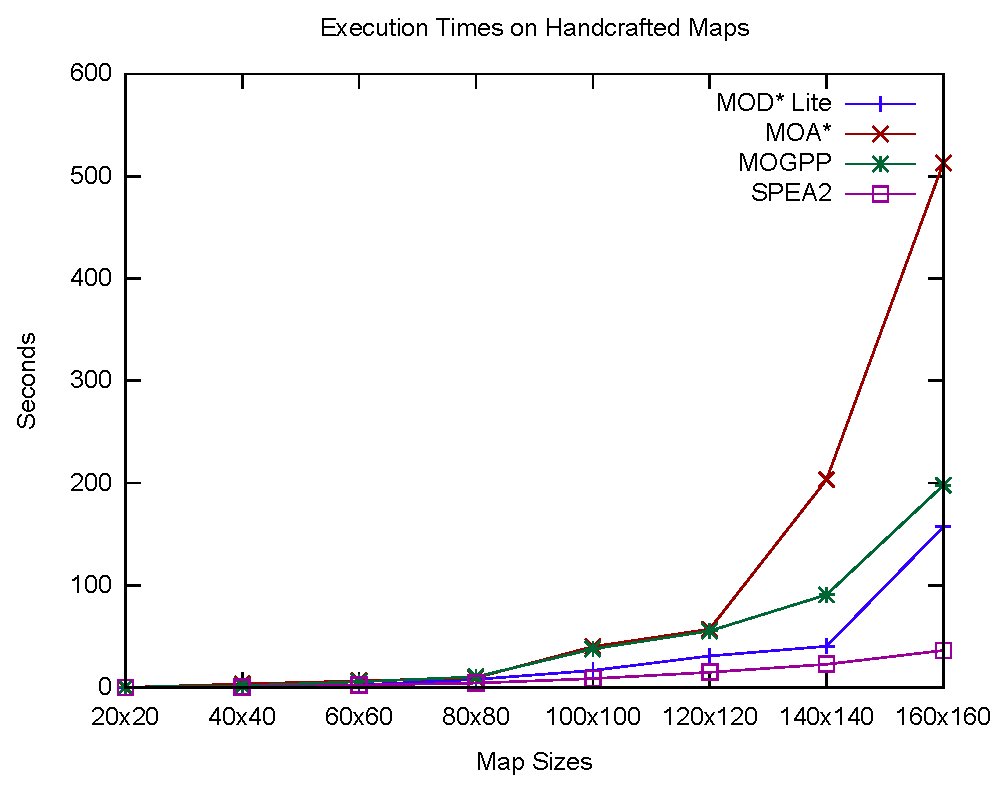
\includegraphics[width=2.1in, angle=270]{handcrafted}
\caption{Execution Times of Handcrafted Fully Observable Maps}
\label{fig:hand_fully}
\end{figure}

\begin{table}[ht]
	\caption{Found Non-dominated Path Costs For Handcrafted Maps}
	\centering
    \begin{tabular}{l l l}
        \hline
        Map Size  &  MOD* Lite  &  MOA* \\ [0.5ex] \hline
        25 x 25   &  (49, 722)  &  (49, 722) 
		   \cr    &  (51, 505)   &  (51, 505)
   		   \cr    &  (55, 216)   &  (55, 216) \\ 
        50 x 50   & (99, 14)   & (99, 14)
		   \cr	  &	(101, 0)   &  (101, 0) \\ 
        75 x 75   & (149, 1927) & (149, 1927) 
		   \cr	  &  (151, 1329) & (151, 1329)
		   \cr	  &  (153, 279)	&	(153, 279)
   		   \cr	  &  (159, 0)	&	(159, 0) \\
        100 x 100 & (199, 1077) & (199, 144) 
		   \cr	  & (201, 20) & (201, 20)
		   \cr	  & (205, 0) & (205, 0)\\
        125 x 125 & (249, 15) & (249, 15)
		   \cr    & 			 & (257, 0) \\
        150 x 150 & (301, 20) & (299, 145)
    		   \cr	  & 			 & (301, 20) 
   		   \cr	  & 		  & (315, 0) \\ [1ex]
        \hline
    \end{tabular}
	\label{table:handPaths}
\end{table}

In the second set of tests, we construct handcrafted maps with same sizes, threat zone and obstacle ratio with randomized tests as indicated above. These maps are also assumed fully observable and agent's initial and target locations are taken randomly. All handcrafted test environments \textit{guarantee} that at least two non-dominated paths will be available. Execution times are shown in Figure \ref{fig:hand_fully} and generated paths' costs are given in Table \ref{table:handPaths}. In both set of tests, it can be seen that MOA* consumes exponentially increased times to find optimal solutions especially when map sizes increase.

\begin{figure}
\centering
\includegraphics[width=2.1in, angle=270]{75x75ThreatZonePercent}
\caption{75x75 Fully Observable Map on Different Threat Zones}
\label{fig:tzratio}
\end{figure}

%\begin{figure*}[htbp]
%\begin{center}$
%\begin{array}{cc}
%\includegraphics[width=1.9in, angle=270]{75x75SensorRange}
%\includegraphics[width=1.9in, angle=270]{100x100SensorRange} \\
%\includegraphics[width=1.9in, angle=270]{125x125SensorRange}
%\end{array}$
%\end{center}
%\caption{Sensor Ranges on Different Maps}
%\label{fig:sensorRanges}
%\end{figure*}

\begin{figure}
\centering
\includegraphics[width=2.0in, angle=270]{75x75SensorRange}
\caption{Sensor Ranges on a 75x75 Map}
\label{fig:sensorRanges1}
\end{figure}

\begin{figure}
\centering
\includegraphics[width=2.0in, angle=270]{100x100SensorRange}
\caption{Sensor Ranges on a 100x100 Map}
\label{fig:sensorRanges2}
\end{figure}

\begin{figure}
\centering
\includegraphics[width=2.0in, angle=270]{125x125SensorRange}
\caption{Sensor Ranges on a 125x125 Map}
\label{fig:sensorRanges3}
\end{figure}


As we use threat zones and their risk values as the second objective, percentages of these zones also effect execution time and generated path quality. Different threat zone percents are also tested on a fully observable 75 x 75 map and results are given in Figure \ref{fig:tzratio}. We could say that increasing risks of threat zones  does not effect performance of  MOD* Lite much, it finds results on approximately near times. However, MOA* tightly coupled with it and execution time increases gradually as the threat percentage increases.

%\begin{figure}
%\label{fig:75x75sensor}
%\centering
%\includegraphics[width=2.5in, angle=270]{75x75SensorRange}
%\caption{75x75 Partially Observable Map on Different Sensor Ranges}
%\end{figure}

%\begin{figure}
%\label{fig:100x100sensor}
%\centering
%\includegraphics[width=2.5in, angle=270]{100x100SensorRange}
%\caption{100x100 Partially Observable Map on Different Sensor Ranges}
%\end{figure}

%\begin{figure}
%\label{fig:125x125sensor}
%\centering
%\includegraphics[width=2.5in, angle=270]{125x125SensorRange}
%\caption{125x125 Partially Observable Map on Different Sensor Ranges}
%\end{figure}

In fourth set of tests, we generate partially observable randomized maps of sizes 75 x 75, 100 x 100 and 125x125. On these maps, agent's initial and target locations are chosen to be the furthermost cells in the environment. For each map, we set agent' s sensor range from 20\% to 60\% and observe execution times. In these tests, the agent starts to plan a path towards the nearest available cell within its sensor range -the temporary target- to the actual target with respect to manhattan distance. After planning, consider that agent has found three paths with costs $(15, 200)$, $(18, 230)$ and $(23, 260)$. In such cases, the agent tends to choose the path with cost $(18, 230)$, the median of paths. This strategy is independent from algorithm and could be set explicitly according to the domain that algorithm works on. Afterwards, it starts to follow the chosen path. When new cells are available or a weight of a cell is changed within sensor range, agent reassigns the temporary target and re-executes path planner algorithm. This process iterates until the agent reaches to the desired target location.

The fundamental advantage of MOD* Lite can be seen very clearly on these tests. While MOD* Lite has the capability of updating only the effected states due to its incremental nature, MOA* re-plans the overall path from scratch when new parts become known and the weights of some cells have changed. This situation causes MOA* to work on exponentially long times. Total execution times to reach to the target for these test cases are given in Figures \ref{fig:sensorRanges1}, \ref{fig:sensorRanges2} and \ref{fig:sensorRanges3}. As can be seen from results, MOD* Lite can easily handle the dynamical issues of the environment where MOA* fails. Due to discovering different parts of the environment during execution, actual traversed path's costs of MOD* Lite and MOA* might be slightly different from each other, where MOD* Lite could follow a better path with respect to MOA* or vice versa.


\section{Conclusions \& Future Work}
In this paper, we present MOD* Lite, a novel approach for searching, planning and finding paths on known and unknown dynamic environments where the agent needs to optimize more than one criteria that cannot be transformed to each other. MOD* Lite is based on D* Lite and brings multi-objectivity to the solution space successfully, which is required in many real-world problems. Experimental results show that MOD* Lite is able to optimize path quality and is fast enough to be used in real-world multi-agent applications such as robotics, computer games, or virtual simulations. To our best knowledge, MOD* Lite is the first incremental search algorithm to handle multi-objectivity. We are planning to extend MOD* Lite for moving targets. 

\bibliographystyle{ieeetr}
\bibliography{modstar_iat2012}

\end{document}